\documentclass{beamer}
%SAND 2021-7549 O
\usepackage{comment}
\usepackage{color}
\usepackage{listings}
\usepackage{verbatim}
\usepackage{multicol}
\usepackage{booktabs}
\definecolor{green}{RGB}{0,128,0}

\def\EQ#1\EN{\begin{equation*}#1\end{equation*}}
\def\BA#1\EA{\begin{align*}#1\end{align*}}
\def\BS#1\ES{\begin{split*}#1\end{split*}}
\newcommand{\bc}{\begin{center}}
\newcommand{\ec}{\end{center}}
\newcommand{\eq}{\ =\ }
\newcommand{\degc}{$^\circ$C}

\def\p{\partial}
\def\qbs{\boldsymbol{q}}
\def\Dbs{\boldsymbol{D}}
\def\A{\mathcal A}
\def\gC{\mathcal C}
\def\gD{\mathcal D}
\def\gL{\mathcal L}
\def\M{\mathcal M}
\def\P{\mathcal P}
\def\Q{\mathcal Q}
\def\gR{\mathcal R}
\def\gS{\mathcal S}
\def\X{\mathcal X}
\def\bnabla{\boldsymbol{\nabla}}
\def\bnu{\boldsymbol{\nu}}
\renewcommand{\a}{{\alpha}}
%\renewcommand{\a}{{}}
\newcommand{\s}{{\sigma}}
\newcommand{\bq}{\boldsymbol{q}}
\newcommand{\bz}{\boldsymbol{z}}
\def\bPsi{\boldsymbol{\Psi}}

\def\Li{\textit{L}}
\def\Fb{\textbf{f}}
\def\Jb{\textbf{J}}
\def\cb{\textbf{c}}

\def\Dt{\Delta t}
\def\tpdt{{t + \Delta t}}
\def\bpsi{\boldsymbol{\psi}}
\def\dbpsi{\delta \boldsymbol{\psi}}
\def\bc{\textbf{c}}
\def\dbc{\delta \textbf{c}}
\def\arrows{\rightleftharpoons}

\newcommand{\bGamma}{\boldsymbol{\Gamma}}
\newcommand{\bOmega}{\boldsymbol{\Omega}}
%\newcommand{\bPsi}{\boldsymbol{\Psi}}
%\newcommand{\bpsi}{\boldsymbol{\psi}}
\newcommand{\bO}{\boldsymbol{O}}
%\newcommand{\bnu}{\boldsymbol{\nu}}
\newcommand{\bdS}{\boldsymbol{dS}}
\newcommand{\bg}{\boldsymbol{g}}
\newcommand{\bk}{\boldsymbol{k}}
%\newcommand{\bq}{\boldsymbol{q}}
\newcommand{\br}{\boldsymbol{r}}
\newcommand{\bR}{\boldsymbol{R}}
\newcommand{\bS}{\boldsymbol{S}}
\newcommand{\bu}{\boldsymbol{u}}
\newcommand{\bv}{\boldsymbol{v}}
%\newcommand{\bz}{\boldsymbol{z}}
\newcommand{\pressure}{P}

\def\water{H$_2$O}
\def\calcium{Ca$^{2+}$}
\def\copper{Cu$^{2+}$}
\def\magnesium{Mg$^{2+}$}
\def\sodium{Na$^+$}
\def\potassium{K$^+$}
\def\uranium{UO$_2^{2+}$}
\def\hion{H$^+$}
\def\hydroxide{0H$^-$}
\def\bicarbonate{HCO$_3^-$}
\def\carbonate{CO$_3^{2-}$}
\def\cotwo{CO$_2$(aq)}
\def\chloride{Cl$^-$}
\def\fluoride{F$^-$}
\def\phosphoricacid{HPO$_4^{2-}$}
\def\nitrate{NO$_3^-$}
\def\sulfate{SO$_4^{2-}$}
\def\souotwooh{$>$SOUO$_2$OH}
\def\sohuotwocothree{$>$SOHUO$_2$CO$_3$}
\def\soh{$>$SOH}

\newcommand\gehcomment[1]{{{\color{orange} #1}}}
\newcommand\add[1]{{{\color{blue} #1}}}
\newcommand\remove[1]{\sout{{\color{red} #1}}}
\newcommand\codecomment[1]{{{\color{green} #1}}}
\newcommand\redcomment[1]{{{\color{red} #1}}}
\newcommand\bluecomment[1]{{{\color{blue} #1}}}
\newcommand\greencomment[1]{{{\color{green} #1}}}
\newcommand\magentacomment[1]{{{\color{magenta} #1}}}

\begin{comment}
\tiny
\scriptsize
\footnotesize
\small
\normalsize
\large
\Large
\LARGE
\huge
\Huge
\end{comment}

\begin{document}
\title{1D Multicontinuum Transport \ldots in a Nutshell}
\author{Rosie Leone }
\date{\today}

%\frame{\titlepage}


%-----------------------------------------------------------------------------
\section{Description of a 1D Tracer Multicontinuum Model}

\subsection{1D Multicontinuum Transport Model}

\frame{\frametitle{Description of 1D Tracer Multicontinuum Scenario}
The ``1D Multicontinuum Transport Model'' simulates solute transport within a 10 m single fracture with matrix diffusion in a 1 m 1D matrix:
\begin{itemize}
  \item Problem domain: $10 \times 1 \times 1$ m$^3$ ($x \times y \times z$)
  \item Grid resolution $100 \times 1 \times 1$ m$^3$ ($100 \times$ 1 $\times$ 1 cells)
  \item Secondary domain: 1 m
  \item Secondary grid cells per primary: 50
  \item Maximum time step size: 1.0 d
  \item Total simulation time: 500 d
\end{itemize}

}

%-----------------------------------------------------------------------------
\frame{\frametitle{1D Tracer Multicontinuum Scenario Schematic}
\begin{itemize}
  \item Transport in fracture due to advection and dispersion
  \item Transport in matrix due to diffusion only
\end{itemize}

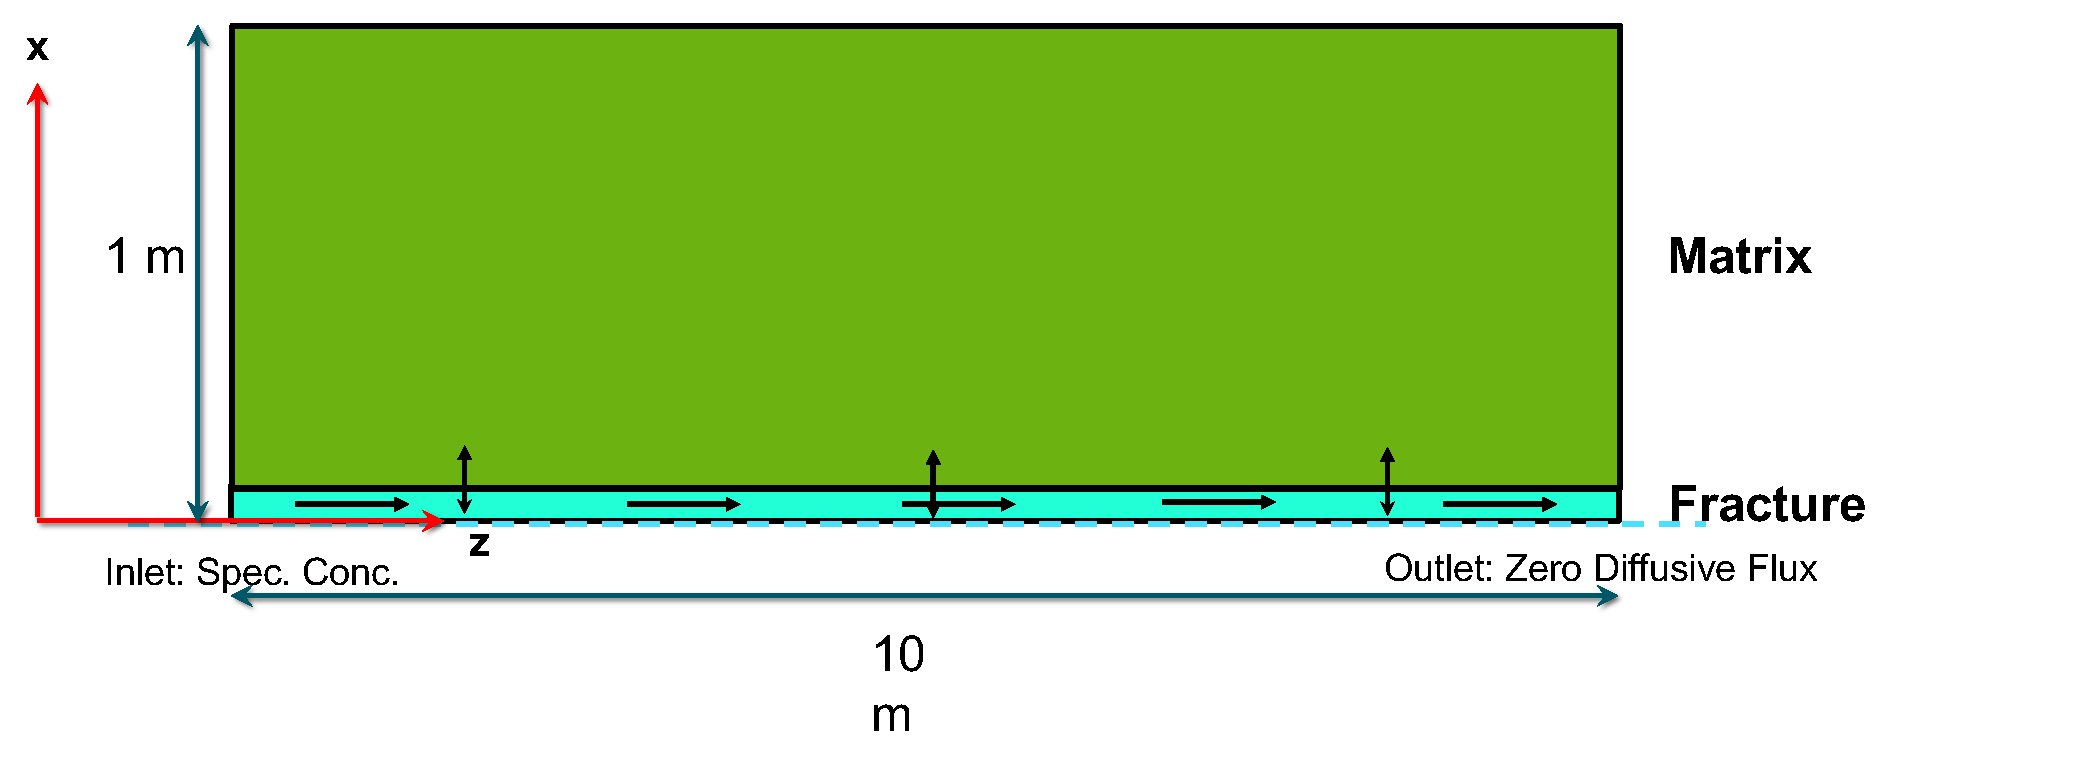
\includegraphics[width=\linewidth]{./slab_fig}
}

%-----------------------------------------------------------------------------
\subsection{Governing Equations
}
\frame{\frametitle{Governing Reactive Transport Equations}

%\Large

\EQ\label{primary}
\frac{\p}{\p t} \left(\varepsilon_f \varphi_f s \Psi_j^f\right) + \bnabla\cdot\bOmega_j^f \eq
-\sum_f A_{fm} \Psi_j^{fm} - \varepsilon_f \sum_k \nu_{jk} \Gamma_k^f - \varepsilon_f \frac{\p S_j^f}{\p t}
\EN

\EQ\label{secondary}
\frac{\p}{\p t} \left(\varphi_f s \Psi_j^m\right) + \bnabla_\xi\cdot\bOmega_j^m \eq
- \sum_k \nu_{jk} \Gamma_k^m - \frac{\p S_j^m}{\p t}
\EN

\EQ\label{bc}
\Psi_{jk}^{fm} \left(r,t\right) = \Psi_{jk}^m \left(\xi_{fm},t\mid r\right)
\EN

%\bigskip
%\normalsize
\footnotesize
\begin{align*}
\varphi_f &\eq \text{porosity in fracture}; \quad
\varphi_m \eq \text{porosity in matrix}\\
\Psi &\eq \text{total component concentration}\\
\epsilon_f &\eq \text{Fracture volume fraction} \\
\bOmega &\eq \text{solute flux} \\
A_{fm} &\eq \text{fracture-matrix interfacial area} \\
\sum_k \nu_{jk} \Gamma_k^f &\eq \text{mineral reaction}\\
\xi &\eq \text{generalized coordinate}
\end{align*}

}

%-----------------------------------------------------------------------------
\section{Description of Input Deck}

\subsection{SIMULATION}

\begin{frame}[fragile,containsverbatim]\frametitle{SIMULATION}

\begin{itemize}
  \item Decaying solute transport with matrix diffusion
\end{itemize}

\begin{semiverbatim}
SIMULATION
  SIMULATION_TYPE SUBSURFACE
  PROCESS_MODELS
    SUBSURFACE_TRANSPORT transport
      MODE GIRT
      \magentacomment{OPTIONS
        MULTIPLE_CONTINUUM
      /}
    /
  /
END

SUBSURFACE
  ...
END_SUBSURFACE
\end{semiverbatim}

\end{frame}

%-----------------------------------------------------------------------------
\begin{frame}[fragile,containsverbatim]\frametitle{GRID}

\begin{itemize}
  \item Problem domain: $10 \times 1 \times 1$ m (x $\times$ y $\times$ z)
  \item Grid resolution $100 \times 1 \times 1$ m
\end{itemize}

\begin{semiverbatim}
GRID
  TYPE structured
  NXYZ 100 1 1
  BOUNDS
    0.d0 0.d0 0.d0
    10.d0 1.d0 1.d0
  /
END
\end{semiverbatim}

\end{frame}

%-----------------------------------------------------------------------------
\subsection{REGION}

\begin{frame}[fragile,containsverbatim,allowframebreaks]\frametitle{REGION}

\begin{itemize}
  \item Delineate regions for:
  \begin{itemize}
    \item entire domain
    \item west boundary face
    \item east boundary face
  \end{itemize}
\end{itemize}

\begin{semiverbatim}
REGION all
  COORDINATES
    0.d0  0.d0 0.d0
    10.d0 1.d0 1.d0
  /
END

\newpage
REGION west        \bluecomment{inflow of domain}
  FACE WEST
  COORDINATES
    0.d0 0.d0 0.d0
    0.d0 1.d0 1.d0
  /
END

REGION east           \bluecomment{outflow of domain}
  FACE EAST
  COORDINATES
    10.d0 0.d0 0.d0
    10.d0 1.d0 1.d0
  /
END

REGION obs      \bluecomment{! point}
  \magentacomment{COORDINATE} 2.d0 0.5d0 0.5d0
END

\end{semiverbatim}

\end{frame}


%-----------------------------------------------------------------------------
\subsection{MATERIAL\_PROPERTY}

\begin{frame}[fragile,containsverbatim]\frametitle{MATERIAL\_PROPERTY}

\begin{itemize}
  \item Add secondary continuum
\end{itemize}

\begin{semiverbatim}
MATERIAL_PROPERTY soil1
  ID 1
  POROSITY 1.d0
  TORTUOSITY 1.d0
  ROCK_DENSITY 2700.d0 #kg/m3
  LONGITUDINAL_DISPERSIVITY 0.5 #m
  \magentacomment{SECONDARY_CONTINUUM
    TYPE SLAB               \bluecomment{! single fracture}
    LENGTH 1.0              \bluecomment{! half fracture spacing [m]}
    AREA 1.0                \bluecomment{! specific surface area [1/m]}
    NUM_CELLS 50            \bluecomment{! secondary cells per primary}
    EPSILON 0.00005d0       \bluecomment{! fracture volume fraction}
    DIFFUSION_COEFFICIENT 1.6d-10  \bluecomment{! includes tortuosity}
    POROSITY 0.01
  / }
END
\end{semiverbatim}

\end{frame}

%-----------------------------------------------------------------------------
\subsection{FLUID\_PROPERTY}

\begin{frame}[fragile,containsverbatim]\frametitle{FLUID\_PROPERTY}

\begin{itemize}
  \item Assign a molecular diffusion coefficient of $10^{-9}$ m$^2$/s
\end{itemize}

\begin{semiverbatim}

FLUID_PROPERTY
  DIFFUSION_COEFFICIENT 1.d-9   \bluecomment{! [m^2/s]}
END
\end{semiverbatim}

\end{frame}

%-----------------------------------------------------------------------------
\subsection{CHEMISTRY}

\begin{frame}[fragile,allowframebreaks]\frametitle{CHEMISTRY}

\begin{itemize}
\item One decaying tracer
\end{itemize}

\begin{semiverbatim}
CHEMISTRY
  PRIMARY_SPECIES
     Tracer
  /
  RADIOACTIVE_DECAY_REACTION
    REACTION Tracer <->
    HALF_LIFE 12.35 y
  /
  LOG_FORMULATION
  DATABASE ../../../database/hanford.dat
  OUTPUT
    All
    TOTAL
  /
END
\end{semiverbatim}

\end{frame}

%-----------------------------------------------------------------------------
\subsection{Miscellaneous}

\begin{frame}[fragile]\frametitle{Miscellaneous}

\begin{itemize}
\item Specify a uniform Darcy velocity of 5d-6 m/d in x-direction
\item Darcy velocity changes as epsilon updates
\end{itemize}


\begin{semiverbatim}

SPECIFIED_VELOCITY
  UNIFORM? YES
  DATASET 5d-6 0.d0 0.d0 m/d
END
\end{semiverbatim}

\end{frame}


%-----------------------------------------------------------------------------
\subsection{TRANSPORT\_CONDITION / CONSTRAINT}

\begin{frame}[fragile,allowframebreaks]\frametitle{TRANSPORT\_CONDITION / CONSTRAINT}

\begin{itemize}
  \item Set up intial condition and inlet boundary condition
\end{itemize}

{
\begin{semiverbatim}

TRANSPORT_CONDITION background
  TYPE ZERO_GRADIENT
    CONSTRAINT_LIST       \bluecomment{! list of constraints}
      0.d0 initial_constraint  
  /
END

TRANSPORT_CONDITION inlet      
  TYPE DIRICHLET
    CONSTRAINT_LIST       \bluecomment{! list of constraints}
      0.d0 inlet_constraint  
  /
END
\end{semiverbatim}
}

\newpage
{\small
\begin{semiverbatim}
CONSTRAINT initial_constraint
  CONCENTRATIONS
    Tracer  1.d-20  T 
  /
/

CONSTRAINT inlet_constraint
  CONCENTRATIONS
    Tracer  1.0  T
  /
/

\magentacomment{SECONDARY_CONSTRAINT sec    \bluecomment{! initial secondary constraint}
  CONCENTRATIONS
    Tracer  1.d-20  T 
  /
/}
\end{semiverbatim}
}

\end{frame}

%-----------------------------------------------------------------------------
\subsection{STRATA}

\begin{frame}[fragile]\frametitle{STRATA}

\begin{itemize}
\item Couple material types with regions
\end{itemize}

\begin{semiverbatim}
STRATA
  REGION all
  MATERIAL soil1
END

\end{semiverbatim}

\end{frame}


%-----------------------------------------------------------------------------
\subsection{OBSERVATION}

\begin{frame}[fragile]\frametitle{OBSERVATION}

\begin{itemize}
\item Couple observation points with regions in model
\end{itemize}

\begin{semiverbatim}
OBSERVATION  \bluecomment{! observation point assigned region name}
  REGION obs  \bluecomment{! region name}
  \magentacomment{SECONDARY_CONCENTRATION}\bluecomment{! output secondary concentration}
END

\end{semiverbatim}

\end{frame}

%-----------------------------------------------------------------------------
\subsection{NUMERICAL METHODS}

\begin{frame}[fragile]\frametitle{NUMERICAL METHODS}

\begin{itemize}
  \item Numerical Methods within subsurface block
  \item Newton Solver sub-block
\end{itemize}

\begin{semiverbatim}
SUBSURFACE

NUMERICAL_METHODS TRANSPORT
  NEWTON_SOLVER
    DTOL 1.d20
  /
END
\end{semiverbatim}

\end{frame}

%-----------------------------------------------------------------------------
\subsection{INITIAL\_CONDITION}

\begin{frame}[fragile]\frametitle{INITIAL\_CONDITION}

\begin{itemize}
\item Couple the \greencomment{initial} transport conditions with region \greencomment{all} for the initial condition
\end{itemize}

\begin{semiverbatim}

INITIAL_CONDITION
  TRANSPORT_CONDITION background
  REGION all
END

\end{semiverbatim}

\end{frame}

%-----------------------------------------------------------------------------
\subsection{BOUNDARY\_CONDITION}

\begin{frame}[fragile,allowframebreaks]\frametitle{BOUNDARY\_CONDITION}

\small
\begin{semiverbatim}
BOUNDARY_CONDITION inlet
  TRANSPORT_CONDITION inlet
  REGION west
END

BOUNDARY_CONDITION outlet
  TRANSPORT_CONDITION background
  REGION east
END

\end{semiverbatim}

\end{frame}

%-----------------------------------------------------------------------------
\subsection{TIME}

\begin{frame}[fragile]\frametitle{TIME}

\begin{itemize}
\item Set final simulation time to 500 days
\item Set initial time step size to 1.e-3 days
\item Set maximum time step size to 1.d0 days
\end{itemize}


\begin{semiverbatim}

TIME
  FINAL_TIME 500.d0 d
  INITIAL_TIMESTEP_SIZE 1.d-3 d
  MAXIMUM_TIMESTEP_SIZE 1.d0 d
END
\end{semiverbatim}

\end{frame}

%-----------------------------------------------------------------------------
\subsection{OUTPUT}

\begin{frame}[fragile]\frametitle{OUTPUT}

\begin{itemize}
\item Print entire solution (a snapshot) in Tecplot format at 100 d and 500 d
\item Print the solution at the observation point for every time step
\end{itemize}

\end{frame}

\begin{frame}[fragile]\frametitle{OUTPUT}

\begin{semiverbatim}\small

OUTPUT
  SNAPSHOT_FILE
    TIMES d 100.
    FORMAT TECPLOT POINT
    NO_PRINT_INITIAL
  /
  OBSERVATION_FILE
    PERIODIC TIMESTEP 1
    PRINT_COLUMN_IDS       \bluecomment{! Adds column ids to obs. header}
  /
  VELOCITY_AT_CENTER       \bluecomment{! include velocities}
END

\end{semiverbatim}

\end{frame}


%-----------------------------------------------------------------------------

\subsection{Running PFLOTRAN}

\begin{frame}[fragile]\frametitle{Running PFLOTRAN}

\begin{semiverbatim}

> cd $PFLOTRAN_DIR
> cd shortcourse/exercises/1D_tracer_multicontinuum
> pflotran -input_prefix tracer_1D_MC
> python conc_in_fracture.py
> python conc_in_matrix.py

\end{semiverbatim}

\end{frame}

%-----------------------------------------------------------------------------
\section{Description of Input Deck: Switch to infiltration}

\subsection{Input File Modifications}

\begin{frame}[fragile]\frametitle{Switch to Infiltration from Matrix with Sorbing Tracer}

Input File Modifications
\begin{itemize}
\item Modify cards:
  \begin{itemize}
    \item CHEMISTRY
    \item CONSTRAINT
   \end{itemize}
\end{itemize}

\end{frame}

%-----------------------------------------------------------------------------
\subsection{CHEMISTRY}

\begin{frame}[fragile]\frametitle{CHEMISTRY}

\begin{itemize}
\item Add in distribution coefficients
\end{itemize}

\begin{semiverbatim}
SORPTION
  ISOTHERM_REACTIONS
    Tracer
      TYPE LINEAR   
      \bluecomment{! Calculating distribution coefficient (Kd)
      ! from retardation (R)
      !   Kd = porosity*saturation*water_density*(R-1)
      !   water_density = 1000. [kg/m^3]
      !   saturation = 1. 
      !   matrix porosity = 0.01 
      ! R = 2, Kd = 10.}
      DISTRIBUTION_COEFFICIENT 0.0 
      SEC_CONT_KD 10.0 kg/m^3   \bluecomment{! kg water/m^3 bulk}
    /
  /
/
\end{semiverbatim}

\end{frame}

%-----------------------------------------------------------------------------
\subsection{CONSTRAINT}

\begin{frame}[fragile]\frametitle{MATERIAL\_PROPERTY}

\begin{itemize}
\item Change primary and secondary concentrations
\end{itemize}

\begin{semiverbatim}
CONSTRAINT inlet_constraint
  CONCENTRATIONS
    Tracer  \magentacomment{1.d-20}  T
  /
/

SECONDARY_CONSTRAINT sec
  CONCENTRATIONS
    Tracer  \magentacomment{1.d0}  T 
  /
/
  
\end{semiverbatim}

\end{frame}

%-----------------------------------------------------------------------------

\subsection{Running PFLOTRAN}

\begin{frame}[fragile]\frametitle{Running PFLOTRAN}

\begin{semiverbatim}

> cd $PFLOTRAN_DIR
> cd shortcourse/exercises/1D_tracer_multicontinuum
> pflotran -input_prefix tracer_1D_MC_leaching
> python conc_fracture_leaching_matrix.py

\end{semiverbatim}

\end{frame}



\end{document}


